\setchapterpreamble[o]{%
  \dictum[James  Magary]{\textit{``Computers can figure  out all  kinds of
      problems, except the things in  the world that just don't add up.''}
  }}

\chapter{Requirements Analysis}
\label{cha:requirements}

This chapter  details on the  goals that were  outlined at the end  of the
previous chapter. To analyze  the requirements to the \gls{glo:XenBEE} the
analysis process is divided into two parts: \emph{Functional Requirements}
and \emph{Non-Functional Requirements}.

The section  on \emph{Functional Requirements}  aims to analyze  the first
two  goals of  this work,  \ie  \emph{Batch job  execution semantics}  and
\emph{On-demand server deployment}.  Both are pure functional requirements
that have  to be  designed and implemented  in the  \gls{glo:XenBEE}. This
section will also contain some additional use cases the are related to the
job  execution.   The provided  use  cases  are  analyzed with  regard  to
\emph{Integrability} of the \gls{glo:XenBEE} into grid-like environments.

The \emph{Non-Functional  Requirements} address the  goals \emph{Security}
and \emph{Efficiency}. Therefore some ideas will be presented that provide
a secure and efficient execution of jobs.

\section{Functional Requirements}
\label{sec:req:functional-requirements}

This section discusses the execution semantics that are to be supported by
the \gls{glo:XenBEE}.   In particular  it analyzes how  batch jobs  can be
executed on  a remote virtual machine  and how server  applications can be
deployed on-demand to virtual machines.

The following sections  describe the execution of these  kind of jobs, but
first of all the basic execution semantics are analyzed.

\subsection{Basic execution semantic}

Suppose you  wanted to execute a  job on a remote  resource. The execution
environment should at least provide the following functions: submission of
a  job,  status  retrieval  and   termination  of  a  submitted  job  (see
Figure~\ref{fig:uc-basic-execution}).

In the \gls{glo:XenBEE} a job  is defined by an \emph{execution container}
along with a description of the  job. The execution container is a virtual
machine image that  contains the application to which  the job refers.

\begin{figure}[ht]
  \centering
  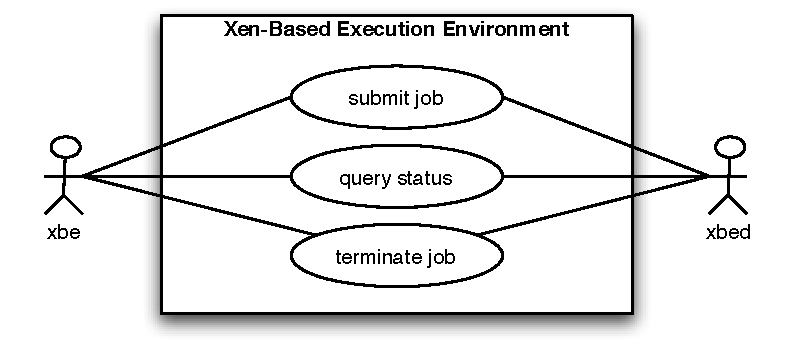
\includegraphics[scale=0.65]{uc-basic-execution}
  \caption{Basic execution semantics.}
  \label{fig:uc-basic-execution}
\end{figure}

The \emph{query status}  use case requires the modeling  of a finite state
automaton that describes the current state of a job (job-state model). The
\gls{glo:OGSA}-\emph{Basic  Execution Service} \cite{ogsa-bes}  provides a
stable, generic and extensible specification for such a job-state model (a
detailed description can be found in Section~\ref{sec:fundamentals:bes} on
page~\pageref{sec:fundamentals:bes}).   To support the  integrability with
grid-like  environments   this  specification   should  be  used   in  the
\gls{glo:XenBEE}.

The  \emph{terminate  job}  use  case  must  always  be  available  to  a
user. That  means a  user must be  able to  terminate the execution  of a
previously submitted job  at any time.  The \emph{terminate  job} use case
is also included in the \gls{glo:BES} state model.

\subsection{Batch job execution}
\label{sec:req:batch-job-execution}

A \emph{batch job} is a program that is executed by a computation resource
without further  user input, \ie  the opposite to  \emph{interactive job}.
Batch jobs  typically transform input  data into output data,  whereas the
input data  may also be  absent. If no  programming errors have  been made
these  kind  of jobs  finish  after an  undefined  but  finite time.   The
execution   of  the   POV-Ray   raytracer  \cite{POV-Ray}   to  render   a
user-supplied scene is an example for this kind of jobs.

Figure~\ref{fig:uc-batch-job-execution}  shows  the  individual use  cases
that are involved when submitting a batch job to the \gls{glo:XenBEE}. The
user has  to provide  the virtual  machine image and  the input  data. The
\emph{\gls{glo:xbed}}  must then access  these files  to create  a virtual
machine that executes  the batch job. The generated output  data has to be
made available by the \emph{xbed} so that the user can access it.

\begin{figure}[ht]
  \centering
  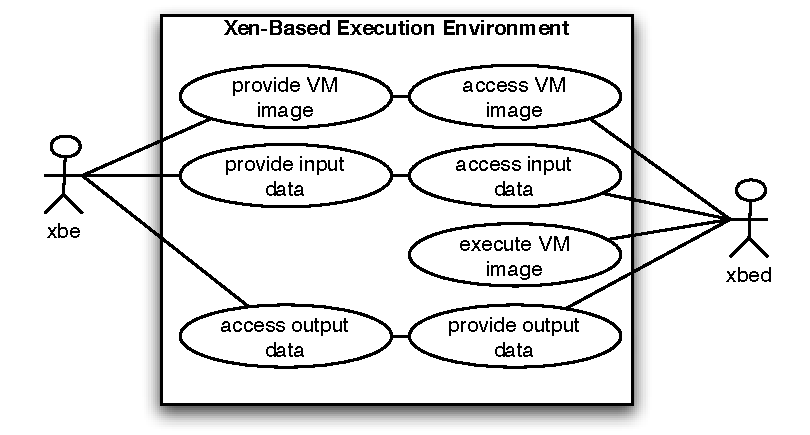
\includegraphics[scale=0.65]{uc-submit-task}
  \caption{Batch job execution use cases.}
  \label{fig:uc-batch-job-execution}
\end{figure}

The  following sections specify  the requirements  for the  job submission
description  and  provide  some  ideas  on  how  an  implementation  could
implement the data access.

\subsubsection{Job description}

The  crucial  part  of  this  use  case is  the  description  of  the  job
submission.     In   the    past   each    grid   middlewares    such   as
Condor~\cite{condor},     Unicore~\cite{unicore}     or     the     Globus
Toolkit~\cite{globus}  used  their  own proprietary  submission  language.
This  made  interoperability  between  different  grids  middlewares  very
difficult.

The   \emph{Job    Submission   Description   Language}   (\gls{glo:JSDL},
\cite{jsdl-spec}) is  generic description  language for the  submission of
computational jobs  to a remote  resource. To the  time of the  writing of
this  work the  mentioned  grid  middlewares have  already  moved to  this
language or are in progress to do so.

Since the \gls{glo:XenBEE} should  be integrable into grid environments, a
fixed requirement  for the \gls{glo:XenBEE} is to  use the \gls{glo:JSDL}.
For     more     information     on     the     \gls{glo:JSDL}     consult
Section~\ref{sec:fundamentals:jsdl}                                      on
page~\pageref{sec:fundamentals:jsdl}.

\subsubsection{Selecting a VM image}

The submission of a task includes  the selection of an image that contains
the application  the user  wants to execute.   A sophisticated  process of
image-selection can  be rather complicated, since it  involves matching of
available  images  against  a  description  provided by  the  user.   Such
selection mechanisms are out of the scope of this thesis.

\subsubsection{File provision and access}

In a preliminary step the client must make the \gls{glo:VM} image, as well
as  the  input data  available  to  the  \emph{xbed}.  The  \gls{glo:JSDL}
supports     \emph{Uniform    Resource     Identifiers}    (\gls{glo:URI},
\cite{rfc2396}) that  can be  used to accomplish  this task, \ie  the user
specifies  the location  of  an  input file  with  a \gls{glo:URI}.   The
\emph{xbed} is then able to access  (retrieve) the files.  The same can be
applied for the provision of generated output data, \ie the user specifies
the target location to which an output file should be uploaded.

\subsubsection{Virtual machine creation}

For each submitted job a new  virtual machine has to be instantiated. This
virtual  machine uses  the \gls{glo:VM}  image provided  by the  user. The
application that is to be executed is specified by the client with the use
of the \gls{glo:JSDL}.

To  actually  execute  the  application  in the  virtual  machine  another
component  is required: the  \emph{\gls{glo:xbeinstd}}. This  component is
then used to control and monitor the execution on the virtual machine.

\subsection{On-demand Server deployment}
\label{sec:req:server-deployment}

A  \emph{server application} or  a \emph{service}  is a  remotely executed
program loops over  the following steps indefinitely often:  wait for user
input, execute a  computation on the input data,  generate output data.  A
web server is  an example for such an application: it  waits until a user
(or  some  service)  makes a  request  to  it,  handles the  request  (\ie
retrieval  of a  document)  and  eventually returns  the  result (\ie  the
document).

\begin{figure}[ht]
  \centering
  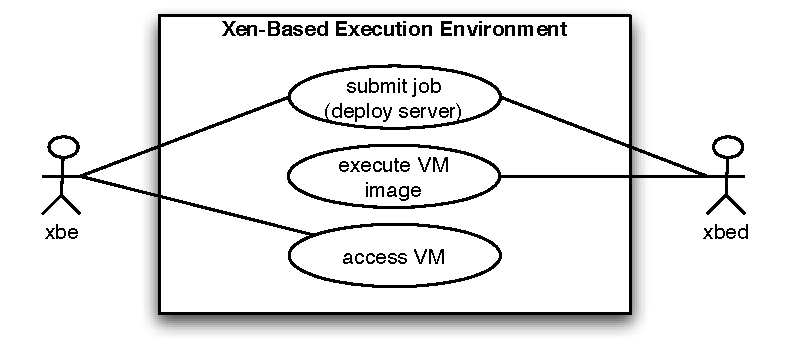
\includegraphics[scale=0.65]{uc-deploy-server}
  \caption{Server deployment use cases.}
  \label{fig:uc-server-deployment}
\end{figure}

The use cases that are  involved in the \emph{on-demand server deployment}
process  are   depicted  in  Figure~\ref{fig:uc-server-deployment}.   This
process shares  most of  the involved use  cases with the  batch execution
process.

In contrast  to a batch job  submission, the virtual  machine instance may
run ``forever'', \ie the ``job''  runs until the \gls{glo:VM} is shut down
by the  user or  the job  itself is terminated.   This must  be explicitly
stated in the job description.

Another difference  is that the  \gls{glo:VM} must be reachable  through a
standard network  connection (\eg TCP/IP  connectivity).  This can  be the
case for  virtual machines that execute  batch jobs, too, but  it need not
to.

Based on the network connectivity, a login to the \gls{glo:VM} can also be
provided.  For  example by  using the \emph{Secure  Shell} (\gls{glo:SSH},
\cite{openssh}).

\subsection{Caching of data}
\label{sec:uc-data-caching}

Imagine a  user who wants to  execute the same  application several times.
That would mean he has to submit  the same image over and over again. This
imposes a  heavy load on the network  that is connecting the  user and the
server. It would  be wise to provide a caching  mechanism, that allows the
user to  store his image  on server-side. According to  the \emph{Locality
  Principle}  \cite{locality-principle},   the  caching  should  decreases
overall execution time,  too.  The involved steps to  cache data are shown
in  Figure~\ref{fig:uc-data-caching}.

\begin{figure}[h]
  \centering
  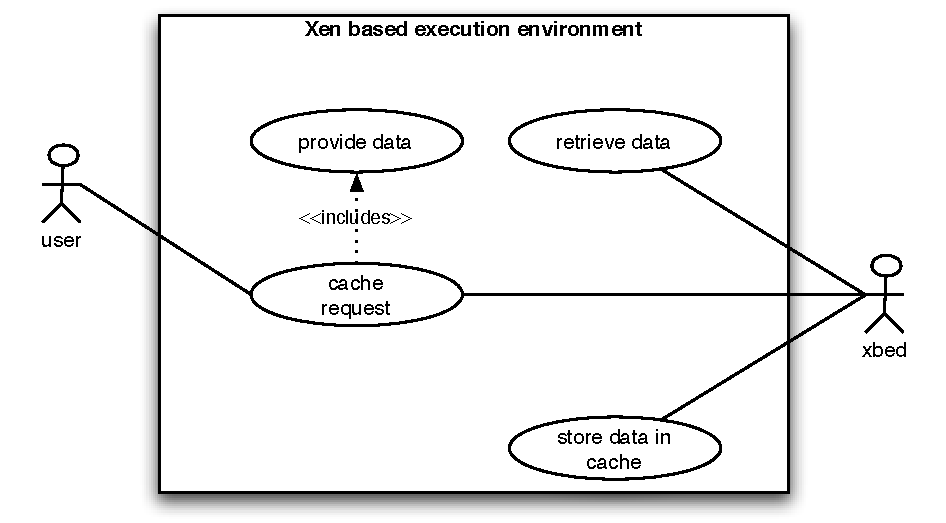
\includegraphics[scale=.75]{uc-data-caching}
  \caption[UC  Data  Caching]{A user  who  is  requesting  the caching  of
    (arbitrary) data.}
  \label{fig:uc-data-caching}
\end{figure}

The  \emph{cache data} use  case can  also make  use of  \gls{glo:URI}s to
refer to  the data.   The \emph{access cache}  use case requires  that the
entries can be \emph{listed}  and \emph{referenced}. The entries should be
specified  as \gls{glo:URI}s,  too.   This makes  them  available for  job
submissions.

To provide shorter execution times, the \gls{glo:XenBEE} should provide a
cache with the following requirements: Arbitrary data must be addable, a
cache listing must be available, cache entries must be indentifiable by
\gls{glo:URI}.

\subsection{Support for Calana}
\label{sec:calana-support}

Calana is a new agent-based  Grid scheduler that uses auctions to schedule
job  submissions.   A  short  description   of  Calana  can  be  found  in
Appendix~\ref{app:sec:calana}    and    in    \cite{dalheimer05agentbased,
  petry06}.

Calana  assumes that  a computation  resource supports  reservations. That
means the resource must  provide semantics to \emph{make}, \emph{confirm},
\emph{use} and \emph{cancel} reservations.

Figure~\ref{fig:calana-xenbee} describes how a  user would interact with a
system, that uses Calana for  job scheduling and the \gls{glo:XenBEE} as a
computation resource. This scenario  requires an agent that implements the
Calana  protocol   on  the  one  hand   and  the  protocol   used  in  the
\gls{glo:XenBEE} on the other hand.

\begin{figure}[htbp]
  \centering
  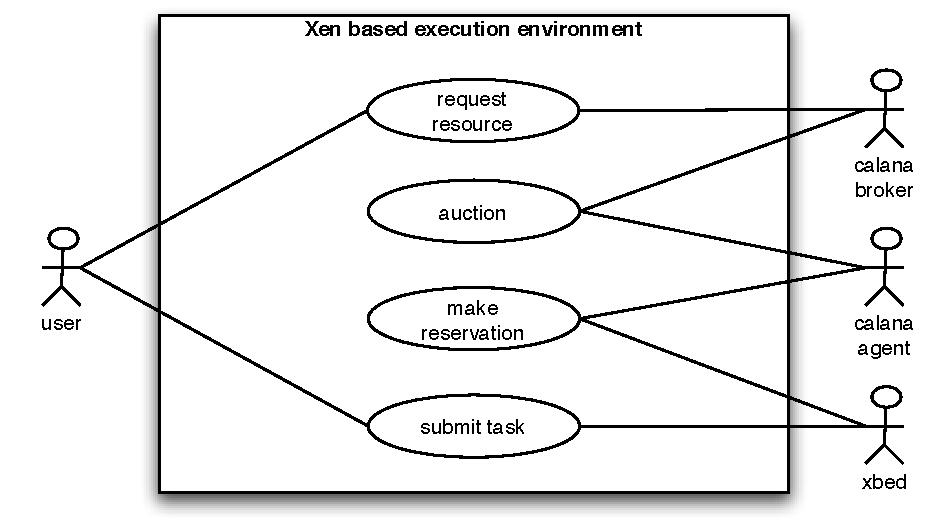
\includegraphics[scale=0.55]{uc-calana-xenbee}
  \caption[Calana and  XenBEE]{The actors and use cases  that are involved
    when a Calana agent uses the \gls{glo:XenBEE} as its resource.}
  \label{fig:calana-xenbee}
\end{figure}

The user requests a resource from the broker which will in turn open up an
auction among  its agents.  One of  those agents are shown  in the figure.
In order  to bid  on the auction  the agent  creates a reservation  on the
\emph{xbed}.   If the auction  is lost,  the reservation  is automatically
canceled.   If the auction  was won,  the user  is eventually  presented a
unique identifier for his reservation.

This reservation can then be used to submit a job to the \emph{xbed}.  The
\emph{xbed} must then check the validity of this identification number.

To support  Calana the \emph{xbed}  has to provide  reservation semantics,
\ie  it must be  possible to  \emph{make}, \emph{confirm},  \emph{use} and
\emph{cancel} reservations.

\section{Non-functional Requirements}

The following sections  describe shortly which non-functional requirements
the \gls{glo:XenBEE} should support.

\subsection{Security}

This  section aims  on  requirements  that are  related  to security.   In
particular  three  requirements  are presented:  \emph{authentication  and
  authorization}, \emph{secure communication} and \emph{secure execution}.

\subsubsection{Authentication and authorization}

Since the \gls{glo:XenBEE} provides a \emph{service}, the provider of this
service   may  want   to  restrict   access   to  a   selected  group   of
\emph{authorized} people.

Before  granting a  user  the  access to  the  execution environment,  the
identity  of  that  user  has  to  be  verified,  \ie  the  user  must  be
\emph{authenticated}. Without authentication  an unauthorized person could
simply pretend to be an authorized person.

\subsubsection{Secure communication}

Secure  communication  between  the  \emph{xbe}  and  the  \emph{xbed}  is
required    to   prevent   \emph{eavesdropping},    \emph{tampering}   and
\emph{message forgery}. 

That means an attacker must  not have the possibility to overhear probably
confidential data  that maybe  included in a  user's job  description, nor
should it be possible that he  can modify or even create new messages that
seem  to come from  this user.

A typical  approach in  Grid middlewares such  as Globus  \cite{globus} or
Unicore   \cite{unicore}   is   to   use  public-key   certificates   (\eg
\gls{glo:X509} certificates) to  provide authentication, authorization and
secure  communication.   The   \gls{glo:XenBEE}  should  follow  the  same
principles.            Section~\ref{sec:secure-communication}           on
page~\ref{sec:secure-communication}   describes   in   detail  how   these
requirements can be provided in the \gls{glo:XenBEE}.

\subsubsection{Secure execution}

This requirement targets at the  actual job execution.  The use of virtual
machines provide  already that  the jobs cannot  harm each  other, because
they are completely separated from each other.

But security has  to be provided on the Xen-host as  well. That means that
data that  belongs to one job (VM  image, input data, output  data, and so
on) must  not be modifiable  or accessible by  any other jobs ---  even if
both jobs belong to the same user.

Since  all files  are accessed  by publicly  reachable  \gls{glo:URI}s, to
ensure the  security of these files  it could be possible  to provide them
encrypted. Before they can be used  by the \emph{xbed} to create a virtual
machine, they have to be decrypted somehow.

\subsection{Efficiency}

Efficiency in the context of  the \gls{glo:XenBEE} means that the overhead
which  is imposed by  the communication  and the  use of  virtual machines
should be kept minimal.

The caching  of virtual machine  images can be  used to decrease  the time
that is  needed to  deploy a  new virtual machine.  This affects  both the
batch  job  execution and  the  on-demand  deployment  of servers  to  key
locations.

% \section{Summary}

% put this figure in the conclusions of this chapter

% \begin{figure}[htbp]
%   \centering
%   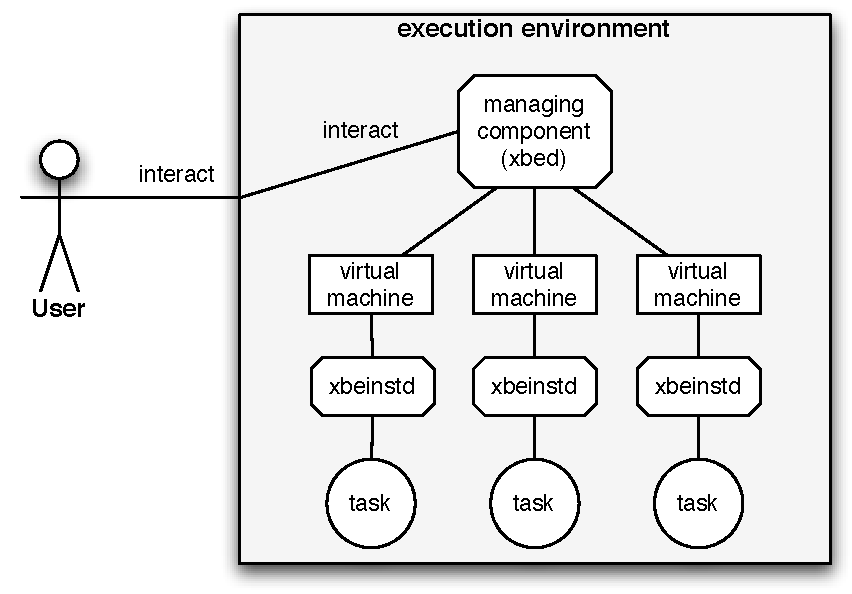
\includegraphics[scale=.7]{concrete-concept}
%   \caption[A more concrete concept]{The  evolved concept, using a managing
%     component (\emph{xbed}) to control the virtual machines.  Each virtual
%     machine  is  dedicated  to  a  single  task  submitted  by  some  user
%     (controlled  through the  \emph{xbeinstd} component).   Users  do only
%     interact with the managing component.}
%   \label{fig:concrete-concept}
% \end{figure}

% \section{A more concrete concept}

% The previous  sections dealt with a  rather abstract view  on the proposed
% execution  environment,  this section  however  outlines  a slightly  more
% concrete  concept  for  the  execution  environment  and  its  components.

% Handling of requests, that the users make to the execution environment and
% controlling the  virtual machines, requires an  additional component. This
% component will be called  \emph{Xen-Based Execution Daemon} or \emph{xbed}
% for short. If a user wants to interact with the execution environment, he
% does  so  by  communicating  directly  with the  managing  component  (see
% Figure~\ref{fig:concrete-concept}).

% Another component which  will be required to control  the actual execution
% of a task  within a virtual machine will  be the \emph{Xen-Based Execution
%   Instance Daemon} or \emph{xbeinstd} for short. There are several reasons
% why this  dedicated component  is required to  be running in  each virtual
% machine. The  most important one is,  that the same  virtual machine image
% could  be used  for more  than just  one application.   Another  reason is
% simply flexibility,  the \gls{glo:JSDL} allows a user  to exactly specify
% how and which application shall be run and this component adheres to that.

% Basically  this concept  defines a  client-server architecture,  where the
% client is represented  by the user (or some mediator  such as a web-portal
% or a  command-line client) and the  server is represented  by the managing
% component.

% The interaction between the users and the execution environment requires a
% communication   layer   over   which    the   requests   are   made.    In
% Section~\ref{sec:fundamentals:mom} I have already introduced \emph{Message
%   Oriented  Middlewares} and  how  message-queue servers  can  be used  to
% provide logical  connections between the  involved distributed components.
% Using the  same concept in this  execution environment makes  sense due to
% the following reasons:

% \begin{itemize}
% \item  There could be  more than  one server  providing such  an execution
%   environment.   Message-queue \emph{topics}\footnote{A \emph{topic}  is a
%     special queue to  which arbitrary many consumers can  subscribe.  If a
%     message gets sent to this  queue, all consumers (rather than just one)
%     receive  this message.}  can  be used  to handle  any number  of those
%   servers uniformly. The clients send  their requests to a single queue on
%   the  \gls{glo:MQS} and  the \gls{glo:MQS}  multiplexes it  to  all known
%   servers.
% \item The server could be in  need of sending messages to clients that are
%   not connected anymore. Think of a notification that could be sent when a
%   task finished its execution.
% \item The use of a MQS renders  it possible that the server can be located
%   behind a very restrictive firewall or even a \gls{glo:NAT}-gateway.
% \item  There is  no visible  difference for  a client,  whether it  uses a
%   direct connection or a connection through a \gls{glo:MQS}.
% \end{itemize}

% The  network  layers  that  are  involved when  using  a  message-oriented
% communication    with    a    message-queue    server   are    shown    in
% Figure~\ref{fig:mqs-layers}.



%%% Local Variables: 
%%% mode: latex
%%% TeX-master: "main.tex"
%%% End: 
